\section{Overview}

This tutorial covers how to estimate divergence times and time calibrated phylogenies. 
The key concepts of this tutorial are node- and fossil-calibrations (assuming a global molecular clock).
A good overview about best practices for node- and fossil-calibrations is found in \cite{Parham2012}, \cite{Warnock2012}, \cite{Joyce2013} and \cite{Warnock2015}.

In this tutorial you will perform a Bayesian inference to estimate a time-calibrated phylogeny.
In the first part we will demonstrate you how to set up a basic model for time-calibrated phylogeny inference.
Throughout we will use the global molecular clock rate.
In a later tutorial we will cover other models for the molecular clock, \EG relaxed clock methods.
The first analysis will use an informative prior distribution on the root age (crown age) to calibrate the phylogeny.
In the second analysis you will use informative node- and fossil-calibrations instead of the informative prior on the root age.
In the third analysis you will use minimum and maximum age constraint (both using hard and soft constraints) to calibrate the phylogeny.
All the assumptions will be covered more in detail later in this tutorial.

\subsection*{Requirements}
We assume that you have read and hopefully completed the following tutorials:
\begin{itemize}
\item RB\_Getting\_Started
\item RB\_Basics\_Tutorial
\item RB\_CTMC\_Tutorial
\end{itemize}
Note that the RB\_Basics\_Tutorial introduces the basic syntax of \Rev but does not cover any phylogenetic models.
You may skip the RB\_Basics\_Tutorial if you have some familiarity with \R.
We tried to keep this tutorial very basic and introduce all the language concepts on the way.
You may only need the RB\_Basics\_Tutorial for a more in-depth discussion of concepts in \Rev.


%%%%%%%%
%%   Data   %%
%%%%%%%%
\section{Data and files}\label{Sec:data}

We provide the data file of DNA sequences required for this tutorial.
You may want to use your own data instead.

\noindent \\ \impmark Create a folder called \cl{data} and download the following files:
\begin{itemize}
\item \href{http://rawgit.com/revbayes/revbayes_tutorial/master/RB_DivergenceTime_Tutorial/data/primates_cytb.nex}{\cl{primates\_cytb.nex}}: Alignment of the \textit{cytochrome b} subunit from 23 primates representing 14 of the 16 families (\textit{Indriidae} and \textit{Callitrichidae} are missing).
\end{itemize}

Below you will also find two tables with the calibration dates that we will use later in this tutorial (see Table~\ref{tab:calibration_perelman} and Table~\ref{tab:calibration_springer}).
Table~\ref{tab:calibration_perelman} will be used for calibrating clades/nodes with informative priors (\EG normal distributions).
Table~\ref{tab:calibration_springer} will be used to calibrate clade/nodes by specifying minimum and maximum ages using hard and soft constraints. 

\begin{table}[tbh!]
\centering
\caption{Node information used for calibrating divergence times in the primate tree from \cite{Perelman2011}.}\label{tab:calibration_perelman}
\begin{tabular}{@{\extracolsep{\fill}}l  c c c r}
\hline
\multicolumn{1}{@{}l}{\textbf{Clade}}  & &\multicolumn{1}{c}{\textbf{Age range (My)}}  & &\multicolumn{1}{c}{\textbf{Citation}} \\ 
\hline
\textit{Simiiformes} & \hspace{2mm} & 43 $\pm$ 4.5 & \hspace{2mm} & \cite{Seiffert2003}\\
\textit{Lorisiformes} & & 40 $\pm$ 3 &  & \cite{Franzen2009,Poux2004}\\
\textit{Catarrhini} & & 29 $\pm$ 6 &  & \cite{Poux2004}\\
\textit{Platyrrhini} & & 23.5 $\pm$ 3 &  & \cite{Hodgson2009,Kay2008}\\
%\textit{Papionini} & & 7 $\pm$ 1 &  & \cite{Steiper2004}\\
\textit{Primates} & & 90 $\pm$ 6 &  & \cite{Matsui2009,Steiper2004,Tavare2002}\\
\hline
\end{tabular}
\end{table}

\begin{table}[tbh!]
\centering
\caption{Calibration intervals used in \cite{Springer2012} to calibrate nodes in the primate tree.}\label{tab:calibration_springer}
\resizebox{\textwidth}{!}{% <------ Don't forget this %
\begin{tabular}{@{\extracolsep{\fill}}l  c c c c c r}
\hline
\multicolumn{1}{@{}l}{\textbf{Clade}}  & &\multicolumn{1}{c}{\textbf{Min Age (My)}}   & &\multicolumn{1}{c}{\textbf{Max Age (My)}}  & &\multicolumn{1}{c}{\textbf{Citation}} \\ 
\hline
\textit{Simiiformes} & \hspace{2mm} & 28.3 &  & 56 & \hspace{2mm} & \cite{Seiffert2003}\\
\textit{Lorisiformes} & & 37.1  & & 56 &  & \cite{Franzen2009,Poux2004}\\
\textit{Catarrhini} & & 20.55 & & 37.3 &  & \cite{Poux2004}\\
\textit{Platyrrhini} & & 11.8 & & 37.3 &  & \cite{Hodgson2009,Kay2008}\\
%\textit{Primates} & & 90 $\pm$ 6 &  & \cite{Matsui2009,Steiper2004,Tavare2002}\\
\hline
\end{tabular}%
}
\end{table}



\newpage
\FloatBarrier
\section{Divergence time estimation using an informative prior on the root age}\label{sec:RootCalibration}

\bigskip
\subsection{Getting Started}



The first section of this exercise involves:
(1) setting up a general time reversible (GTR) substitution model \citep{Tavare1986} with gamma distributed rate variation among sites \citep{Yang1994a} for an alignment of the cytochrome b subunit;
(2) use an informative prior on the root age to date the phylogeny;
(3) approximating the posterior probability of the tree topology and node ages (and all other parameters) using MCMC, and; 
(4) summarizing the MCMC output by computing the maximum \textit{a posteriori} tree. 
This analysis is mostly equivalent to the analysis performed in the RB\_CTMC\_Tutorial.

\begin{figure}[h!]
\centering
\fbox{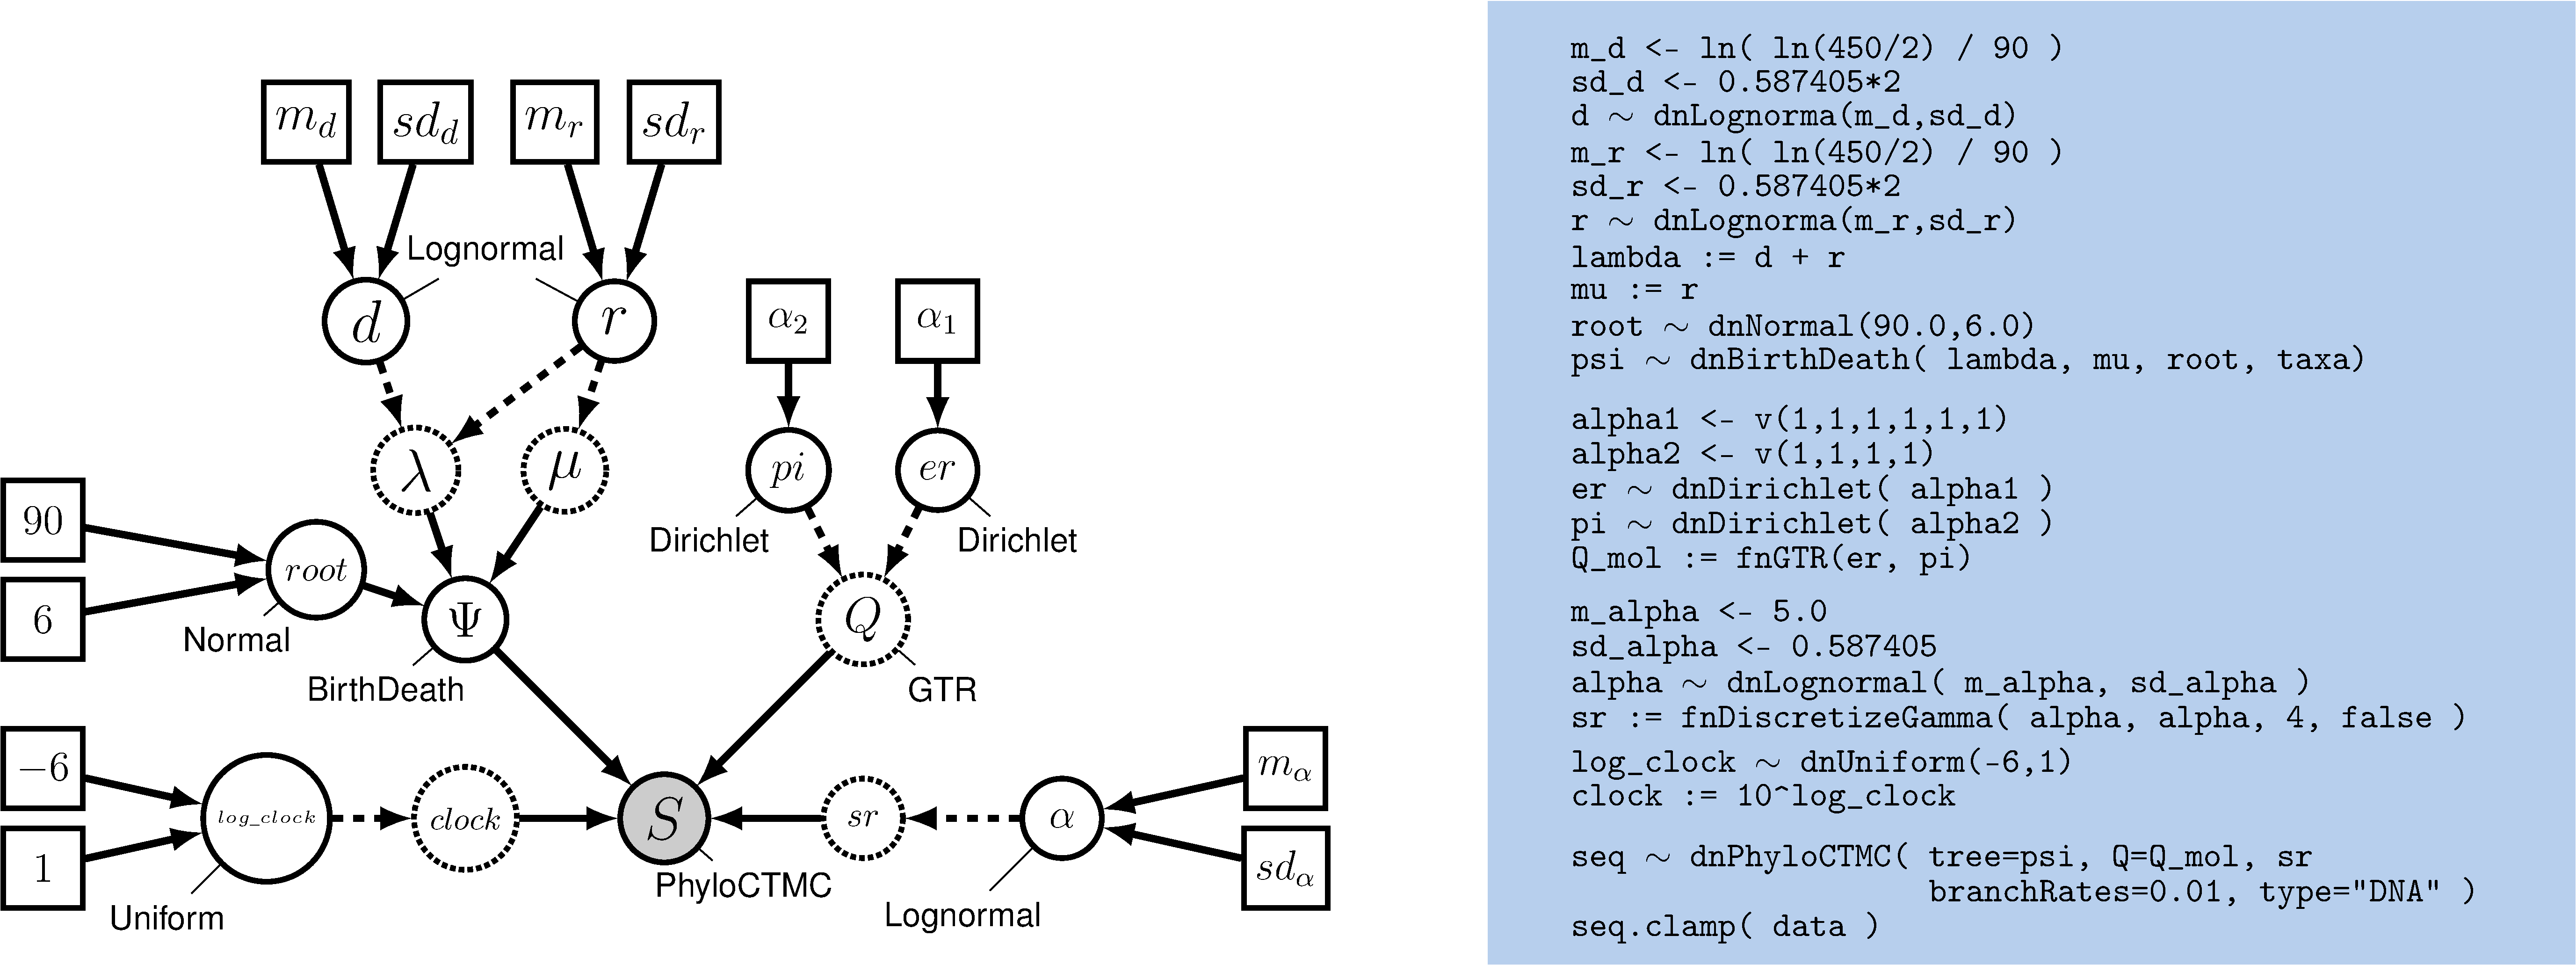
\includegraphics[width=\textwidth,angle=0]{\ResourcePath figures/root_calibration.pdf}}
\caption{\small An example phylogenetic model depicted in graphical-model notation (left) and the corresponding specification in the \Rev language (right).
This example shows the basic outline of the root calibration that we will use in the first exercise.}
\label{fig:clock_prior}
\end{figure}

The general structure of the model is represented in Figure~\ref{fig:clock_prior}.
This figure shows the full model graph.


\bigskip

\subsection{Loading the Data}

\noindent \\ \impmark You should have already downloaded the data files in Section \ref{Sec:data}. 
Links to additional files, including the scripts to run these analyses can be found on the \href{http://revbayes.github.io/tutorials.html}{\RevBayes tutorials website}. 
Remember that the data file should be in a directory called \cl{data} that is in your current working directory.

First load in the sequences using the \cl{readDiscreteCharacterData()} function. 
{\tt \begin{snugshade*}
\begin{lstlisting}
data <- readDiscreteCharacterData("data/primates_cytb.nex")
\end{lstlisting}
\end{snugshade*}}
Executing these lines initializes the data matrix as the respective \Rev variable. 

Next we will specify some useful variables based on our dataset. 
The variable \cl{data} has \textit{member functions} that we can use to retrieve information about the dataset. 
These include the number of species (\cl{n\_species}) and the tip labels (\cl{taxa}).
Each of these variables will be necessary for setting up different parts of our model (\EG the birth-death process prior).
{\tt \begin{snugshade*}
\begin{lstlisting}
n_species <- data.ntaxa()
taxa <- data.taxa()	
\end{lstlisting}
\end{snugshade*}}

Additionally, we set up a counter variable for the number of moves that we already added to our analysis.
[Recall that moves are algorithms used to propose new parameter values during the MCMC simulation.]
This will make it much easier if we extend the model or analysis to include additional moves or to remove some moves.
{\tt \begin{snugshade*}
\begin{lstlisting}
mvi = 0 
\end{lstlisting}
\end{snugshade*}}
You may have noticed that we used the \cl{=} operator to create the move index.
This simply means that the variable is not part of the model.
You will later see that we use this operator more often, \EG when we create moves and monitors.

With the data loaded, we can now proceed to specify our substitution model.



\subsection{General Time Reversible (GTR) Substitution Model}

The GTR model requires that we define and specify a prior on the six exchangeability rates, which we will describe using a flat Dirichlet distribution.
As we did previously for the Dirichlet prior on base frequencies, we first define a constant node specifying the vector of concentration-parameter values using the \cl{v()} function:
{\tt \begin{snugshade*}
\begin{lstlisting}
er_prior <- v(1,1,1,1,1,1) 
\end{lstlisting}
\end{snugshade*}}
This node defines the concentration-parameter values of the Dirichlet prior distribution on the exchangeability rates. 
Now, we can create a stochastic node for the exchangeability rates using the \cl{dnDirichlet()} function, which takes the vector of concentration-parameter values as an argument and the \cl{\rbdn} operator. 
Together, these create a stochastic node named \cl{er}, see Figure~\ref{fig:clock_prior}: 
{\tt \begin{snugshade*}
\begin{lstlisting}
er ~ dnDirichlet(er_prior)
\end{lstlisting}
\end{snugshade*}}
The Dirichlet prior on our parameter \cl{er} creates a \href{http://en.wikipedia.org/wiki/Simplex}{\textit{simplex}} of values that sum to 1. 


For each stochastic node in our model, we must also specify a proposal mechanism if we wish to estimate that parameter. 
{\tt\small \begin{snugshade*}
\begin{lstlisting}
moves[++mvi] = mvSimplexElementScale(er) 
\end{lstlisting}
\end{snugshade*}}

We can use the same type of distribution as a prior on the 4 stationary frequencies ($\pi_A, \pi_C, \pi_G, \pi_T$) since these parameters also represent proportions. 
Specify a flat Dirichlet prior density on the base frequencies:
{\tt \begin{snugshade*}
\begin{lstlisting}
pi_prior <- v(1,1,1,1) 
pi ~ dnDirichlet(pi_prior)
\end{lstlisting}
\end{snugshade*}}

The node \cl{pi} represents the $\pi$ node in Figure~\ref{fig:clock_prior}.
Now add the simplex scale move on the stationary frequencies to the moves vector:
{\tt \small \begin{snugshade*}
\begin{lstlisting}
moves[++mvi] = mvSimplexElementScale(pi)  
\end{lstlisting}
\end{snugshade*}}

We can finish setting up this part of the model by creating a deterministic node for the GTR instantaneous-rate matrix \cl{Q}. 
The \cl{fnGTR()} function takes a set of exchangeability rates and a set of base frequencies to compute the instantaneous-rate matrix used when calculating the likelihood of our model.
{\tt \begin{snugshade*}
\begin{lstlisting}
Q := fnGTR(er,pi)
\end{lstlisting}
\end{snugshade*}}


\subsection{Setting up the Gamma Model}

Create a constant node called \cl{alpha\_prior\_mean} and a second constant node called \cl{alpha\_prior\_sd} for the lognormal prior on the gamma-shape parameter (this is represented as the constant rate parameter in Figure \ref{fig:clock_prior}):
{\tt\begin{snugshade*}
\begin{lstlisting}
alpha_prior_mean <- 5.0
alpha_prior_sd <- 0.587405
\end{lstlisting}
\end{snugshade*}}

Then create a stochastic node called \cl{alpha} with an lognormal prior (this represents the stochastic node for the $\alpha$-shape parameter in Figure \ref{fig:clock_prior}):
{\tt\begin{snugshade*}
\begin{lstlisting}
alpha ~ dnLognormal( alpha_prior_mean, alpha_prior_sd )
\end{lstlisting}
\end{snugshade*}}

The way the ASRV model is implemented involves discretizing the mean-one gamma distribution into a set number of rate categories, $k$. 
To specify this, we need a deterministic node that is a vector that will hold the set of $k$ rates drawn from the gamma distribution with $k$ rate categories. 
The \cl{fnDiscretizeGamma()} function returns this deterministic node and takes three arguments: the shape and rate of the gamma distribution and the number of categories. 
Since we want to discretize a mean-one gamma distribution, we can pass in \cl{alpha} for both the shape and rate.

Initialize the \cl{gamma\_rates} deterministic node vector using the  \cl{fnDiscretizeGamma()} function with \cl{4} bins:
{\tt \begin{snugshade*}
\begin{lstlisting}
gamma_rates := fnDiscretizeGamma( alpha, alpha, 4 )
\end{lstlisting}
\end{snugshade*}}

The random variable that controls the rate variation is the stochastic node \cl{alpha}. 
We will apply a simple scale move to this parameter.
{\tt \begin{snugshade*}
\begin{lstlisting}
moves[++mvi] = mvScale(alpha, weight=2.0)
\end{lstlisting}
\end{snugshade*}}

For more information on ASRV please read the \href{https://github.com/revbayes/revbayes_tutorial/raw/master/tutorial_TeX/RB_CTMC_Tutorial/RB_CTMC_Tutorial.pdf}{RB\_CTMC\_Tutorial}.



\subsection{Tree Prior: Tree Topology and Node Ages}

The tree ( the topology and node ages) is a stochastic node in our phylogenetic model. 
In Figure \ref{fig:clock_prior}, the tree is denoted $\Psi$.
We will assume a constant-rate birth-death process as the prior distribution on the tree.
The distribution in \RevBayes is \cl{dnBDP()}. 
For more information on tree priors please read the \href{https://github.com/revbayes/revbayes_tutorial/raw/master/tutorial_TeX/RB_DiversificationRate_Tutorial/RB_Diversification_Tutorial.pdf}{RB\_DiversificationRate\_Tutorial}.

For the birth-death process we need a speciation rate and extinction rate parameter.
Instead of prior distributions on these parameters directly, we will specify lognormal prior distributions on the diversification and turnover rates.
{\tt \begin{snugshade*}
\begin{lstlisting}
diversification_mean <- ln( ln(n_species/2.0) / 90 )
diversification_sd <- 0.587405*2
diversification ~ dnLognormal(mean=diversification_mean,sd=diversification_sd) 
moves[++mvi] = mvScale(diversification,lambda=1.0,tune=true,weight=3.0)

turnover_mean <- ln( ln(n_species/2.0) / 90 )
turnover_sd <- 0.587405*2
turnover ~ dnLognormal(mean=turnover_mean,sd=turnover_sd) 
moves[++mvi] = mvScale(turnover,lambda=1.0,tune=true,weight=3.0)

### Transform the parameters
birth_rate := diversification + turnover
death_rate := turnover
\end{lstlisting}
\end{snugshade*}}

In our reference publication, \cite{Perelman2011} used a normal distribution with mean of 90.0 MYA with stdev = 6.0 as the prior distribution on the root age.
The normal distribution itself is defined on the complete real line (\IE from $-\infty$ to $+\infty$), however, we know that the root age of primates is definitely larger than 0 (it happen before the present) and smaller than, say, 5000 MYA.
Thus, we truncate the normal distribution.
This also has the advantage that the type of the variable for the root age is a positive real number, instead of a real number.
{\tt \begin{snugshade*}
\begin{lstlisting}
root_time ~ dnNormal(mean=90.0,sd=6.0,min=0.0,max=5000.0)
moves[++mvi] = mvScale(root_time,weight=2.0)
\end{lstlisting}
\end{snugshade*}}

Additionally, we know that we do not have all primate species included in this data set.
We only have 23 out of the approximately 450 primate species.
Thus, we use a sampling fraction to represent this incomplete taxon sampling \citep{Hoehna2011,Hoehna2014a}.
{\tt \begin{snugshade*}
\begin{lstlisting}
rho <- n_species/450
\end{lstlisting}
\end{snugshade*}}

Next, specify the \cl{tree} stochastic node by passing in the tip labels \cl{taxa} to the \cl{dnBDP()} distribution:
{\tt \begin{snugshade*}
\begin{lstlisting}
psi ~ dnBDP(lambda=birth_rate, mu=death_rate, rho=rho, rootAge=root_time, samplingStrategy="uniform", condition="survival", taxa=taxa)
\end{lstlisting}
\end{snugshade*}}

Some types of stochastic nodes can be updated by a number of alternative moves. 
Different moves may explore parameter space in different ways, and it is possible to use multiple different moves for a given parameter to improve mixing (the efficiency of the MCMC simulation). 
In the case of our rooted tree, for example, we can use both a nearest-neighbor interchange move without and with changing the node ages (\cl{mvNarrow} and \cl{mvNNI}) and a fixed-nodeheight subtree-prune and regrafting move (\cl{mvFNPR}). 
For overviews about moves on tree see \cite{Lakner2008}, \cite{Hoehna2008} and \cite{Hoehna2012}.
We also need moves that change the ages of the internal nodes; which are for example the \cl{mvSubtreeScale} and \cl{mvNodeTimeSlideUniform}.
These moves do not have tuning parameters associated with them, thus you only need to pass in the \cl{psi} node and proposal \cl{weight}. 
{\tt \begin{snugshade*}
\begin{lstlisting}
moves[++mvi] = mvNarrow(psi, weight=5.0)
moves[++mvi] = mvNNI(psi, weight=1.0)
moves[++mvi] = mvFNPR(psi, weight=5.0)
moves[++mvi] = mvFNPR(psi, weight=2.0)
moves[++mvi] = mvSubtreeScale(psi, weight=3.0)
moves[++mvi] = mvNodeTimeSlideUniform(psi, weight=15.0)
\end{lstlisting}
\end{snugshade*}}
The weight specifies how often the move will be applied either on average per iteration or relative to all other moves.
Have a look at the MCMC tutorial for more details about moves and MCMC strategies: \href{http://revbayes.github.io/tutorials.html}{http://revbayes.github.io/tutorials.html}

\subsection{Monitoring specific clade ages}

The exercise in this tutorial involves looking at specific age estimates.
There are two ways in \RevBayes how to obtain age estimates.
First, you can look into the generated \emph{maximum a posteriori} tree in \FigTree.
Second, you can add deterministic variables for the ages that you are interested in and look at the values in \Tracer.
Both approaches are useful and could be used together.
For the second approach to work we need to create these deterministic variables.

We start with a deterministic node monitoring the age of the \emph{Catarrhini}.
This involves create a clade object.
A clade object simply contains a number of species names.
Note, the names need to match \textbf{exactly}.
Then, we use the \cl{tmrca} function which will record the \underline{t}ime of the \underline{m}ost \underline{r}ecent \underline{c}ommon \underline{a}ncestor of this clade.
{\tt \begin{snugshade*}
\begin{lstlisting}
clade_catarrhini = clade("Pan_paniscus", "Macaca_mulatta")
age_catarrhini := tmrca(psi, clade_catarrhini)
\end{lstlisting}
\end{snugshade*}}

Next, a deterministic node monitoring the age of the \emph{Platyrrhini}:
{\tt \begin{snugshade*}
\begin{lstlisting}
clade_platyrrhini = clade("Alouatta_palliata", "Callicebus_donacophilus")
age_platyrrhini := tmrca(psi, clade_platyrrhini)
\end{lstlisting}
\end{snugshade*}}

Then, a deterministic node monitoring the age of the \emph{Simiiformes}:
{\tt \begin{snugshade*}
\begin{lstlisting}
clade_simiiformes = clade("Cebus_albifrons", "Macaca_mulatta")
age_simiiformes := tmrca(psi, clade_simiiformes)
\end{lstlisting}
\end{snugshade*}}

And finally, a deterministic node monitoring the age of the \emph{Lorisiformes}:
{\tt \begin{snugshade*}
\begin{lstlisting}
clade_lorisiformes = clade("Loris_tardigradus", "Galago_senegalensis")
age_lorisiformes := tmrca(psi, clade_lorisiformes)
\end{lstlisting}
\end{snugshade*}}


\subsection{The Global Molecular Clock Model}

The global molecular clock assumes that the rate of substitution is constant over the tree and over time (Fig.~\ref{fig:clock_prior}).
Since we calibrated the tree with an informative distribution on the root age we will estimate the clock rate.
Here we use a uniform distribution on the logarithm of the clock rate, which signifies our uncertainty of the magnitude of the clock rate.
We will say that every magnitude or clock rates between $10^{-6}$ and $10^{1}$ are equally probably a priori.
{\tt \begin{snugshade*}
\begin{lstlisting}
logClockRate ~ dnUniform(-6,1)
clockRate := 10^logClockRate

moves[++mvi] = mvSlide(logClockRate)
\end{lstlisting}
\end{snugshade*}}

\subsection{Putting it All Together}

We have fully specified all of the parameters of our phylogenetic model---the tree topology with branch lengths, and the substitution model that describes how the sequence data evolved over the tree with branch lengths.  
Collectively, these parameters comprise a distribution called the \textit{phylogenetic continuous-time Markov chain}, and we use the \cl{PhyloCTMC} constructor function to create this node.
This distribution requires several input arguments: 
(1) the \cl{tree} with branch lengths; 
(2) the instantaneous-rate matrix \cl{Q};
(3) the clock rate, and; 
(4) the \cl{type} of character data.


Build the random variable for the character data (sequence alignment).
{\tt \begin{snugshade*}
\begin{lstlisting}
# the sequence evolution model
seq ~ dnPhyloCTMC(tree=psi, Q=Q, branchRates=clockRate, siteRates=gamma_rates, type="DNA")
\end{lstlisting}
\end{snugshade*}}


Once the \cl{PhyloCTMC} model has been created, we can attach our sequence data to the tip nodes in the tree.
{\tt \begin{snugshade*}
\begin{lstlisting}
seq.clamp(data)
\end{lstlisting}
\end{snugshade*}}
[Note that although we assume that our sequence data are random variables---they are realizations of our phylogenetic model---for the purposes of inference, we assume that the sequence data are ``clamped''.]
When this function is called, \RevBayes~sets each of the stochastic nodes representing the tips of the tree to the corresponding nucleotide sequence in the alignment. 
This essentially tells the program that we have observed data for the sequences at the tips. 

Finally, we wrap the entire model to provide convenient access to the DAG. 
To do this, we only need to give the \cl{model()} function a single node. 
With this node, the \cl{model()} function can find all of the other nodes by following the arrows in the graphical model:
{\tt \begin{snugshade*}
\begin{lstlisting}
mymodel = model(Q)
\end{lstlisting}
\end{snugshade*}}

\bigskip
\subsection{Performing an MCMC Analysis Under the Global Clock Model}

In this section, will describe how to set up the MCMC sampler and summarize the resulting posterior distribution of trees. 

\subsubsection{Specifying Monitors}

For our MCMC analysis, we need to set up a vector of \textit{monitors} to record the states of our Markov chain. 
The monitor functions are all called \cl{mn*}, where \cl{*} is the wildcard representing the monitor type.
First, we will initialize the model monitor using the \cl{mnModel} function. This creates a new monitor variable that will output the states for all model parameters when passed into a MCMC function. 
{\tt \begin{snugshade*}
\begin{lstlisting}
monitors[++mni] = mnModel(filename="output/primates_cytb_root_calibration.log",printgen=10, separator = TAB)
\end{lstlisting}
\end{snugshade*}}

The \cl{mnFile} monitor will record the states for only the parameters passed in as arguments. We use this monitor to specify the output for our sampled trees and branch lengths.

{\tt \begin{snugshade*}
\begin{lstlisting}
monitors[++mni] = mnFile(filename="output/primates_cytb_root_calibration.trees",printgen=10, separator = TAB, psi)
\end{lstlisting}
\end{snugshade*}}


Finally, create a screen monitor that will report the states of specified variables to the screen with \cl{mnScreen}:
{\tt \begin{snugshade*}
\begin{lstlisting}
monitors[++mni] = mnScreen(printgen=1000, clockRate, root_time, age_simiiformes)
\end{lstlisting}
\end{snugshade*}}

\subsubsection{Initializing and Running the MCMC Simulation}

With a fully specified model, a set of monitors, and a set of moves, we can now set up the MCMC algorithm that will sample parameter values in proportion to their posterior probability. The \cl{mcmc()} function will create our MCMC object:
{\tt \begin{snugshade*}
\begin{lstlisting}
mymcmc = mcmc(mymodel, monitors, moves)
\end{lstlisting}
\end{snugshade*}}


We may wish to run the \cl{.burnin()} member function.
% if we wish to pre-run the chain and discard the initial states. 
% I think you might want to add a brief explanation here, something like:
Recall that this function \textbf{does not} specify the number of states that we wish to discard from the MCMC analysis as burnin (\IE the samples collected before the chain converges to the stationary distribution).  
Instead, the \cl{.burnin()} function specifies a \textit{completely separate} preliminary MCMC analysis that is used to tune the scale of the moves to improve mixing of the MCMC analysis.
{\tt \begin{snugshade*}
\begin{lstlisting}
mymcmc.burnin(generations=10000,tuningInterval=250)
\end{lstlisting}
\end{snugshade*}}


Now, run the MCMC:
{\tt \begin{snugshade*}
\begin{lstlisting}
mymcmc.run(generations=30000)
\end{lstlisting}
\end{snugshade*}}

When the analysis is complete, you will have the monitored files in your output directory.

\noindent \\ \impmark Look at the file called \cl{output/primates\_cytb\_root\_calibration.log} in \texttt{Tracer}.


\subsection{Exercise 1}

We are interested in the divergence time estimate between \emph{Simiiformes}, \emph{Platyrrhini}, \emph{Catarrhini}, \emph{Lorisiformes} and all primates.

To obtain an estimate of the divergence time we read in the tree trace and build the annotated maximum \textit{a posteriori} tree.
{\tt \begin{snugshade*}
\begin{lstlisting}
treetrace = readTreeTrace("output/primates_cytb_root_calibration.trees",
                             treetype="clock")
mapTree(treetrace,"output/primates_cytb_root_calibration.tree")
\end{lstlisting}
\end{snugshade*}}
Fill in the following table as you go through the tutorial.

\noindent \\ \impmark Look at the file called \cl{output/primates\_cytb\_root\_calibration.tree} in \texttt{FigTree}.


\begin{Form}
\begin{table}[h!]
\centering
\caption{\small Estimated divergence times in our primates example$^*$.}
\resizebox{\textwidth}{!}{% <------ Don't forget this %
\begin{tabular}{l c c c c c c c c c c c}
\hline
\multicolumn{1}{l}{\textbf{ }} &\multicolumn{1}{r}{\textbf{ }} & \multicolumn{2}{c}{\textbf{Primates}}  & \multicolumn{2}{c}{\textbf{Simiiformes}} & \multicolumn{2}{c}{\textbf{Platyrrhini}} & \multicolumn{2}{c}{\textbf{Catarrhini}} & \multicolumn{2}{c}{\textbf{Lorisiformes}} \\ 
\cline{3-12}
\multicolumn{1}{l}{\textbf{Clock Model}} & \multicolumn{1}{r}{\hspace{3mm}} & \multicolumn{1}{c}{\textit{Mean Estimate}} & \multicolumn{1}{c}{\textit{Credible interval}} & \multicolumn{1}{c}{\textit{Mean Estimate}} & \multicolumn{1}{c}{\textit{Credible interval}} & \multicolumn{1}{c}{\textit{Mean Estimate}} & \multicolumn{1}{c}{\textit{Credible interval}} & \multicolumn{1}{c}{\textit{Mean Estimate}} & \multicolumn{1}{c}{\textit{Credible interval}} & \multicolumn{1}{c}{\textit{Mean Estimate}} & \multicolumn{1}{c}{\textit{Credible interval}} \\ 
\hline
\ref{sec:RootCalibration} Root Calibration & \hspace{15mm} & \TextField[name=m1,backgroundcolor={.85 .85 .85},color={1 0 0},height=4ex]{}  & \TextField[name=ml2,backgroundcolor={.85 .85 .85},color={0 0 1},height=4ex]{} & \TextField[name=m3,backgroundcolor={.85 .85 .85},color={1 0 0},height=4ex]{}  & \TextField[name=ml4,backgroundcolor={.85 .85 .85},color={0 0 1},height=4ex]{} & \TextField[name=m5,backgroundcolor={.85 .85 .85},color={1 0 0},height=4ex]{}  & \TextField[name=ml6,backgroundcolor={.85 .85 .85},color={0 0 1},height=4ex]{} & \TextField[name=m7,backgroundcolor={.85 .85 .85},color={1 0 0},height=4ex]{}  & \TextField[name=ml8,backgroundcolor={.85 .85 .85},color={0 0 1},height=4ex]{} & \TextField[name=m9,backgroundcolor={.85 .85 .85},color={1 0 0},height=4ex]{}  & \TextField[name=ml10,backgroundcolor={.85 .85 .85},color={0 0 1},height=4ex]{}\\
\hline
\ref{sec:NodeCalibration} Node Calibration & \hspace{3mm} &\TextField[name=ml11,backgroundcolor={.85 .85 .85},color={1 0 0},height=4ex]{} & \TextField[name=ml12,backgroundcolor={.85 .85 .85},color={0 0 1},height=4ex]{} & \TextField[name=m13,backgroundcolor={.85 .85 .85},color={1 0 0},height=4ex]{}  & \TextField[name=ml14,backgroundcolor={.85 .85 .85},color={0 0 1},height=4ex]{} & \TextField[name=m15,backgroundcolor={.85 .85 .85},color={1 0 0},height=4ex]{}  & \TextField[name=ml16,backgroundcolor={.85 .85 .85},color={0 0 1},height=4ex]{} & \TextField[name=m17,backgroundcolor={.85 .85 .85},color={1 0 0},height=4ex]{}  & \TextField[name=ml18,backgroundcolor={.85 .85 .85},color={0 0 1},height=4ex]{} & \TextField[name=m19,backgroundcolor={.85 .85 .85},color={1 0 0},height=4ex]{}  & \TextField[name=ml20,backgroundcolor={.85 .85 .85},color={0 0 1},height=4ex]{} \\
\hline
\ref{sec:HardBounds} Hard Bounds& \hspace{3mm} &\TextField[name=ml21,backgroundcolor={.85 .85 .85},color={1 0 0},height=4ex]{} & \TextField[name=ml22,backgroundcolor={.85 .85 .85},color={0 0 1},height=4ex]{} & \TextField[name=m23,backgroundcolor={.85 .85 .85},color={1 0 0},height=4ex]{}  & \TextField[name=ml24,backgroundcolor={.85 .85 .85},color={0 0 1},height=4ex]{} & \TextField[name=m25,backgroundcolor={.85 .85 .85},color={1 0 0},height=4ex]{}  & \TextField[name=ml26,backgroundcolor={.85 .85 .85},color={0 0 1},height=4ex]{} & \TextField[name=m27,backgroundcolor={.85 .85 .85},color={1 0 0},height=4ex]{}  & \TextField[name=ml28,backgroundcolor={.85 .85 .85},color={0 0 1},height=4ex]{} & \TextField[name=m29,backgroundcolor={.85 .85 .85},color={1 0 0},height=4ex]{}  & \TextField[name=ml30,backgroundcolor={.85 .85 .85},color={0 0 1},height=4ex]{}  \\
\hline
\ref{sec:SoftBounds} Soft Bounds & \hspace{3mm} &\TextField[name=ml31,backgroundcolor={.85 .85 .85},color={1 0 0},height=4ex]{} & \TextField[name=ml32,backgroundcolor={.85 .85 .85},color={0 0 1},height=4ex]{} & \TextField[name=m33,backgroundcolor={.85 .85 .85},color={1 0 0},height=4ex]{}  & \TextField[name=ml34,backgroundcolor={.85 .85 .85},color={0 0 1},height=4ex]{} & \TextField[name=m35,backgroundcolor={.85 .85 .85},color={1 0 0},height=4ex]{}  & \TextField[name=ml36,backgroundcolor={.85 .85 .85},color={0 0 1},height=4ex]{} & \TextField[name=m37,backgroundcolor={.85 .85 .85},color={1 0 0},height=4ex]{}  & \TextField[name=ml38,backgroundcolor={.85 .85 .85},color={0 0 1},height=4ex]{} & \TextField[name=m39,backgroundcolor={.85 .85 .85},color={1 0 0},height=4ex]{}  & \TextField[name=ml40,backgroundcolor={.85 .85 .85},color={0 0 1},height=4ex]{}  \\
\hline
{\footnotesize{$^*$you can edit this table}}\\
\end{tabular}%
}
\label{tab:divergence_times}
\end{table}
\end{Form}




\newpage
\section{Informative node calibration}\label{sec:NodeCalibration}

In the previous section we calibrated the phylogeny using an informative prior on the root age only.
This part of the exercise will involve specifying a informative prior on internal nodes in our tree: 
(1) \emph{Semiiformes}, the split between \emph{New World Monkeys} and \emph{OldWorld Monkeys}; 
(2) \emph{Platyrrhini};
(3) \emph{Catarrhini}; and 
(4) \emph{Lorisifomres}, the split between \emph{galagids} and \emph{lorisids}.

In \RevBayes, calibrated internal nodes are treated differently than in many other programs for estimating species divergence times (\EG BEAST).
This is because the graphical model structure used in \RevBayes does not allow a stochastic node to be assigned more than one prior distribution. 
By contrast, the common approach to applying calibration densities as used in other dating softwares leads to incoherence in the calibration prior \citep[for detailed explainations of this see][]{Warnock2012,Heled2012,Heath2014}. 
More explicitly, common calibration approaches assume that the age of a calibrated node is modeled by the tree-wide diversification process (\EG birth-death model) \emph{and} a parametric density parameterized by the occurrence time of a fossil (or other external prior information).
This can induce a calibration prior density that is not consistent with the birth-death process or the parametric prior distribution. 
Thus, approaches that condition the birth-death process on the calibrated nodes are more statistically coherent \citep{Yang2006}.

In \RevBayes, calibration densities are applied in a different way, treating fossil observation times like data. 
The graphical model in Figure \ref{m_BDCal:fig} illustrates how calibrated nodes are specified in the directed acyclic graph (DAG).
Here, the age of the calibration node (\IE the internal node specified as the MRCA of the fossil and a set of living species) is a deterministic node---\EG denoted $o_1$ for fossil $\mathcal{F}_1$---and acts as an offset on the stochastic node representing the age of the fossil specimen.
The fossil age, $\mathcal{F}_i$, is specified as a stochastic node and clamped to its \emph{observed} age in the fossil record. 
The node $\mathcal{F}_i$ is modeled using a distribution that describes the waiting time from the speciation event to the appearance of the observed fossil. 
Thus, if the MCMC samples any state of $\Psi$ for which the age of $\mathcal{F}_i$ has a probability of 0, then that state will always be rejected, effectively calibrating the birth-death process without applying multiple prior densities to any calibrated node (Fig.~\ref{m_BDCal:fig}).


%\begin{figure}[h!]
%\centering
%\fbox{\includegraphics[width=6in]{\ResourcePath figures/calib_BDR_gm.eps}}
%\caption{\small The graphical model representation of the node-calibrated birth-death process in \RevBayes.}
%\label{m_BDCal:fig}
%\end{figure}

\subsection{Adding node calibrations}
Additional to the model that we used in the previous exercise we will add calibrations to some clades (see Table~\ref{tab:calibration_perelman}).

First, we specify the calibration for the catarrhini split using a normal distribution with mean 29 and standard deviation of 6.
{\tt \begin{snugshade*}
\begin{lstlisting}
obs_age_catarrhini ~ dnNormal(age_catarrhini,6)
obs_age_catarrhini.clamp(29)
\end{lstlisting}
\end{snugshade*}}

Next, we specify the calibration for the Platyrrhini split using a normal distribution with mean 23.5 and standard deviation of 3.
{\tt \begin{snugshade*}
\begin{lstlisting}
obs_age_platyrrhini ~ dnNormal(age_platyrrhini,3)
obs_age_platyrrhini.clamp(23.5)
\end{lstlisting}
\end{snugshade*}}

Then, we specify the calibration for the split between \emph{New World Monkeys} and \emph{OldWorld Monkeys}  using a normal distribution with mean 43 and standard deviation of 4.5.
{\tt \begin{snugshade*}
\begin{lstlisting}
obs_age_simiiformes ~ dnNormal(age_simiiformes,4.5)
obs_age_simiiformes.clamp(43)
\end{lstlisting}
\end{snugshade*}}

Finally, we specify the calibration for the lorisiformes (the split between \emph{galagids} and \emph{lorisids}) using a normal distribution with mean 40 and standard deviation of 3.
{\tt \begin{snugshade*}
\begin{lstlisting}
obs_age_lorisiformes ~ dnNormal(age_lorisiformes,3)
obs_age_lorisiformes.clamp(40)
\end{lstlisting}
\end{snugshade*}}


\subsection{Exercise 2}

\begin{itemize}
\item Copy the file \cl{RootCalibration.Rev} and call it \cl{NodeCalibration}.
\item Add the node calibrations outlines above.
\item Rename the output files (\IE the filenames for the monitors).
\item Run the MCMC analysis.
\item Look at the output in \Tracer.
\item Fill in the table.
\end{itemize}




\newpage
\section{Hard-bounded node calibrations}\label{sec:HardBounds}
Additional to the model that we used in the previous exercise we will add calibrations to some clades (see Table~\ref{tab:calibration_springer}).

First, we specify the calibration for the catarrhini split using a uniform distribution with minimum of 20.55 and maximum of 37.3.
{\tt \begin{snugshade*}
\begin{lstlisting}
min_age_catarrhini <- 20.55
max_age_catarrhini <- 37.3
width_age_prior_catarrhini <- (max_age_catarrhini-min_age_catarrhini)/2.0
mean_age_prior_catarrhini <- min_age_catarrhini + width_age_prior_catarrhini
obs_age_catarrhini ~ dnUniform(age_catarrhini - width_age_prior_catarrhini, age_catarrhini + width_age_prior_catarrhini)
obs_age_catarrhini.clamp( mean_age_prior_catarrhini )
\end{lstlisting}
\end{snugshade*}}

Next, we specify the calibration for the Platyrrhini split using a uniform distribution with minimum of 11.8 and maximum of 37.3.
{\tt \begin{snugshade*}
\begin{lstlisting}
min_age_platyrrhini <- 11.8
max_age_platyrrhini <- 37.3
width_age_prior_platyrrhini <- (max_age_platyrrhini-min_age_platyrrhini)/2.0
mean_age_prior_platyrrhini <- min_age_platyrrhini + width_age_prior_platyrrhini
obs_age_platyrrhini ~ dnUniform(age_platyrrhini - width_age_prior_platyrrhini, age_platyrrhini + width_age_prior_platyrrhini)
obs_age_platyrrhini.clamp( mean_age_prior_platyrrhini )
\end{lstlisting}
\end{snugshade*}}

Then, we specify the calibration for the split between \emph{New World Monkeys} and \emph{OldWorld Monkeys} using a uniform distribution with minimum of 28.3 and maximum of 56.
{\tt \begin{snugshade*}
\begin{lstlisting}
min_age_simiiformes <- 28.3
max_age_simiiformes <- 56
width_age_prior_simiiformes <- (max_age_simiiformes-min_age_simiiformes)/2.0
mean_age_prior_simiiformes <- min_age_simiiformes + width_age_prior_simiiformes
obs_age_simiiformes ~ dnUniform(age_simiiformes - width_age_prior_simiiformes, age_simiiformes + width_age_prior_simiiformes)
obs_age_simiiformes.clamp( mean_age_prior_simiiformes )
\end{lstlisting}
\end{snugshade*}}

Finally, we specify the calibration for the lorisiformes (the split between \emph{galagids} and \emph{lorisids}) using a uniform distribution with minimum of 37.1 and maximum of 56.
{\tt \begin{snugshade*}
\begin{lstlisting}
min_age_lorisiformes <- 37.1
max_age_lorisiformes <- 56
width_age_prior_lorisiformes <- (max_age_lorisiformes-min_age_lorisiformes)/2.0
mean_age_prior_lorisiformes <- min_age_lorisiformes + width_age_prior_lorisiformes
obs_age_lorisiformes ~ dnUniform(age_lorisiformes - width_age_prior_lorisiformes, age_lorisiformes + width_age_prior_lorisiformes)
obs_age_lorisiformes.clamp( mean_age_prior_lorisiformes )
\end{lstlisting}
\end{snugshade*}}


\subsection{Exercise 3}

\begin{itemize}
\item Copy the file \cl{RootCalibration.Rev} and call it \cl{HardBoundsNodeCalibration.Rev}.
\item Add the node calibrations outlines above.
\item Rename the output files (\IE the filenames for the monitors).
\item Run the MCMC analysis.
\item Look at the output in \Tracer.
\item Fill in the table.
\end{itemize}





\newpage
\section{Soft-bounded node calibrations}\label{sec:SoftBounds}
Additional to the model that we used in the previous exercise we will add calibrations to some clades (see Table~\ref{tab:calibration_springer}).

First, we specify the calibration for the catarrhini split using a uniform distribution with minimum of 20.55 and maximum of 37.3.
{\tt \begin{snugshade*}
\begin{lstlisting}
min_age_catarrhini <- 20.55
max_age_catarrhini <- 37.3
width_age_prior_catarrhini <- (max_age_catarrhini-min_age_catarrhini)/2.0
mean_age_prior_catarrhini <- min_age_catarrhini + width_age_prior_catarrhini
obs_age_catarrhini ~ dnSoftBoundUniformNormal(min=age_catarrhini - width_age_prior_catarrhini, max=age_catarrhini + width_age_prior_catarrhini, sd=2.5, p=0.95)
obs_age_catarrhini.clamp( mean_age_prior_catarrhini )
\end{lstlisting}
\end{snugshade*}}

Next, we specify the calibration for the Platyrrhini split using a uniform distribution with minimum of 11.8 and maximum of 37.3.
{\tt \begin{snugshade*}
\begin{lstlisting}
min_age_platyrrhini <- 11.8
max_age_platyrrhini <- 37.3
width_age_prior_platyrrhini <- (max_age_platyrrhini-min_age_platyrrhini)/2.0
mean_age_prior_platyrrhini <- min_age_platyrrhini + width_age_prior_platyrrhini
obs_age_platyrrhini ~ dnSoftBoundUniformNormal(min=age_platyrrhini - width_age_prior_platyrrhini, max=age_platyrrhini + width_age_prior_platyrrhini, sd=2.5, p=0.95)
obs_age_platyrrhini.clamp( mean_age_prior_platyrrhini )
\end{lstlisting}
\end{snugshade*}}

Then, we specify the calibration for the split between \emph{New World Monkeys} and \emph{OldWorld Monkeys} using a uniform distribution with minimum of 28.3 and maximum of 56.
{\tt \begin{snugshade*}
\begin{lstlisting}
min_age_simiiformes <- 28.3
max_age_simiiformes <- 56
width_age_prior_simiiformes <- (max_age_simiiformes-min_age_simiiformes)/2.0
mean_age_prior_simiiformes <- min_age_simiiformes + width_age_prior_simiiformes
obs_age_simiiformes ~ dnSoftBoundUniformNormal(min=age_simiiformes - width_age_prior_simiiformes, max=age_simiiformes + width_age_prior_simiiformes, sd=2.5, p=0.95)
width_age_prior_simiiformes)
obs_age_simiiformes.clamp( mean_age_prior_simiiformes )
\end{lstlisting}
\end{snugshade*}}

Finally, we specify the calibration for the lorisiformes (the split between \emph{galagids} and \emph{lorisids}) using a uniform distribution with minimum of 37.1 and maximum of 56.
{\tt \begin{snugshade*}
\begin{lstlisting}
min_age_lorisiformes <- 37.1
max_age_lorisiformes <- 56
width_age_prior_lorisiformes <- (max_age_lorisiformes-min_age_lorisiformes)/2.0
mean_age_prior_lorisiformes <- min_age_lorisiformes + width_age_prior_lorisiformes
obs_age_lorisiformes ~ dnSoftBoundUniformNormal(min=age_lorisiformes - width_age_prior_lorisiformes, max=age_lorisiformes + width_age_prior_lorisiformes, sd=2.5, p=0.95)
width_age_prior_lorisiformes)
obs_age_lorisiformes.clamp( mean_age_prior_lorisiformes )
\end{lstlisting}
\end{snugshade*}}


\subsection{Exercise 4}

\begin{itemize}
\item Copy the file \cl{RootCalibration.Rev} and call it \cl{SoftBoundsNodeCalibration.Rev}.
\item Add the node calibrations outlines above.
\item Rename the output files (\IE the filenames for the monitors).
\item Run the MCMC analysis.
\item Look at the output in \Tracer.
\item Fill in the table.
\end{itemize}


\bibliographystyle{sysbio}
\bibliography{\GlobalResourcePath refs}
